% Options for packages loaded elsewhere
\PassOptionsToPackage{unicode}{hyperref}
\PassOptionsToPackage{hyphens}{url}
%
\documentclass[
  man]{apa6}
\usepackage{amsmath,amssymb}
\usepackage{iftex}
\ifPDFTeX
  \usepackage[T1]{fontenc}
  \usepackage[utf8]{inputenc}
  \usepackage{textcomp} % provide euro and other symbols
\else % if luatex or xetex
  \usepackage{unicode-math} % this also loads fontspec
  \defaultfontfeatures{Scale=MatchLowercase}
  \defaultfontfeatures[\rmfamily]{Ligatures=TeX,Scale=1}
\fi
\usepackage{lmodern}
\ifPDFTeX\else
  % xetex/luatex font selection
\fi
% Use upquote if available, for straight quotes in verbatim environments
\IfFileExists{upquote.sty}{\usepackage{upquote}}{}
\IfFileExists{microtype.sty}{% use microtype if available
  \usepackage[]{microtype}
  \UseMicrotypeSet[protrusion]{basicmath} % disable protrusion for tt fonts
}{}
\makeatletter
\@ifundefined{KOMAClassName}{% if non-KOMA class
  \IfFileExists{parskip.sty}{%
    \usepackage{parskip}
  }{% else
    \setlength{\parindent}{0pt}
    \setlength{\parskip}{6pt plus 2pt minus 1pt}}
}{% if KOMA class
  \KOMAoptions{parskip=half}}
\makeatother
\usepackage{xcolor}
\usepackage{graphicx}
\makeatletter
\def\maxwidth{\ifdim\Gin@nat@width>\linewidth\linewidth\else\Gin@nat@width\fi}
\def\maxheight{\ifdim\Gin@nat@height>\textheight\textheight\else\Gin@nat@height\fi}
\makeatother
% Scale images if necessary, so that they will not overflow the page
% margins by default, and it is still possible to overwrite the defaults
% using explicit options in \includegraphics[width, height, ...]{}
\setkeys{Gin}{width=\maxwidth,height=\maxheight,keepaspectratio}
% Set default figure placement to htbp
\makeatletter
\def\fps@figure{htbp}
\makeatother
\setlength{\emergencystretch}{3em} % prevent overfull lines
\providecommand{\tightlist}{%
  \setlength{\itemsep}{0pt}\setlength{\parskip}{0pt}}
\setcounter{secnumdepth}{-\maxdimen} % remove section numbering
% Make \paragraph and \subparagraph free-standing
\ifx\paragraph\undefined\else
  \let\oldparagraph\paragraph
  \renewcommand{\paragraph}[1]{\oldparagraph{#1}\mbox{}}
\fi
\ifx\subparagraph\undefined\else
  \let\oldsubparagraph\subparagraph
  \renewcommand{\subparagraph}[1]{\oldsubparagraph{#1}\mbox{}}
\fi
\newlength{\cslhangindent}
\setlength{\cslhangindent}{1.5em}
\newlength{\csllabelwidth}
\setlength{\csllabelwidth}{3em}
\newlength{\cslentryspacingunit} % times entry-spacing
\setlength{\cslentryspacingunit}{\parskip}
\newenvironment{CSLReferences}[2] % #1 hanging-ident, #2 entry spacing
 {% don't indent paragraphs
  \setlength{\parindent}{0pt}
  % turn on hanging indent if param 1 is 1
  \ifodd #1
  \let\oldpar\par
  \def\par{\hangindent=\cslhangindent\oldpar}
  \fi
  % set entry spacing
  \setlength{\parskip}{#2\cslentryspacingunit}
 }%
 {}
\usepackage{calc}
\newcommand{\CSLBlock}[1]{#1\hfill\break}
\newcommand{\CSLLeftMargin}[1]{\parbox[t]{\csllabelwidth}{#1}}
\newcommand{\CSLRightInline}[1]{\parbox[t]{\linewidth - \csllabelwidth}{#1}\break}
\newcommand{\CSLIndent}[1]{\hspace{\cslhangindent}#1}
\ifLuaTeX
\usepackage[bidi=basic]{babel}
\else
\usepackage[bidi=default]{babel}
\fi
\babelprovide[main,import]{english}
% get rid of language-specific shorthands (see #6817):
\let\LanguageShortHands\languageshorthands
\def\languageshorthands#1{}
% Manuscript styling
\usepackage{upgreek}
\captionsetup{font=singlespacing,justification=justified}

% Table formatting
\usepackage{longtable}
\usepackage{lscape}
% \usepackage[counterclockwise]{rotating}   % Landscape page setup for large tables
\usepackage{multirow}		% Table styling
\usepackage{tabularx}		% Control Column width
\usepackage[flushleft]{threeparttable}	% Allows for three part tables with a specified notes section
\usepackage{threeparttablex}            % Lets threeparttable work with longtable

% Create new environments so endfloat can handle them
% \newenvironment{ltable}
%   {\begin{landscape}\centering\begin{threeparttable}}
%   {\end{threeparttable}\end{landscape}}
\newenvironment{lltable}{\begin{landscape}\centering\begin{ThreePartTable}}{\end{ThreePartTable}\end{landscape}}

% Enables adjusting longtable caption width to table width
% Solution found at http://golatex.de/longtable-mit-caption-so-breit-wie-die-tabelle-t15767.html
\makeatletter
\newcommand\LastLTentrywidth{1em}
\newlength\longtablewidth
\setlength{\longtablewidth}{1in}
\newcommand{\getlongtablewidth}{\begingroup \ifcsname LT@\roman{LT@tables}\endcsname \global\longtablewidth=0pt \renewcommand{\LT@entry}[2]{\global\advance\longtablewidth by ##2\relax\gdef\LastLTentrywidth{##2}}\@nameuse{LT@\roman{LT@tables}} \fi \endgroup}

% \setlength{\parindent}{0.5in}
% \setlength{\parskip}{0pt plus 0pt minus 0pt}

% Overwrite redefinition of paragraph and subparagraph by the default LaTeX template
% See https://github.com/crsh/papaja/issues/292
\makeatletter
\renewcommand{\paragraph}{\@startsection{paragraph}{4}{\parindent}%
  {0\baselineskip \@plus 0.2ex \@minus 0.2ex}%
  {-1em}%
  {\normalfont\normalsize\bfseries\itshape\typesectitle}}

\renewcommand{\subparagraph}[1]{\@startsection{subparagraph}{5}{1em}%
  {0\baselineskip \@plus 0.2ex \@minus 0.2ex}%
  {-\z@\relax}%
  {\normalfont\normalsize\itshape\hspace{\parindent}{#1}\textit{\addperi}}{\relax}}
\makeatother

% \usepackage{etoolbox}
\makeatletter
\patchcmd{\HyOrg@maketitle}
  {\section{\normalfont\normalsize\abstractname}}
  {\section*{\normalfont\normalsize\abstractname}}
  {}{\typeout{Failed to patch abstract.}}
\patchcmd{\HyOrg@maketitle}
  {\section{\protect\normalfont{\@title}}}
  {\section*{\protect\normalfont{\@title}}}
  {}{\typeout{Failed to patch title.}}
\makeatother

\usepackage{xpatch}
\makeatletter
\xapptocmd\appendix
  {\xapptocmd\section
    {\addcontentsline{toc}{section}{\appendixname\ifoneappendix\else~\theappendix\fi\\: #1}}
    {}{\InnerPatchFailed}%
  }
{}{\PatchFailed}
\keywords{cognitive aging, Rescorla Wagner, spreading activation, network science, }
\DeclareDelayedFloatFlavor{ThreePartTable}{table}
\DeclareDelayedFloatFlavor{lltable}{table}
\DeclareDelayedFloatFlavor*{longtable}{table}
\makeatletter
\renewcommand{\efloat@iwrite}[1]{\immediate\expandafter\protected@write\csname efloat@post#1\endcsname{}}
\makeatother
\usepackage{lineno}

\linenumbers
\usepackage{csquotes}
\ifLuaTeX
  \usepackage{selnolig}  % disable illegal ligatures
\fi
\IfFileExists{bookmark.sty}{\usepackage{bookmark}}{\usepackage{hyperref}}
\IfFileExists{xurl.sty}{\usepackage{xurl}}{} % add URL line breaks if available
\urlstyle{same}
\hypersetup{
  pdftitle={An enrichment account of cognitive aging},
  pdfauthor={Thomas Hills1},
  pdflang={en-EN},
  pdfkeywords={cognitive aging, Rescorla Wagner, spreading activation, network science,},
  hidelinks,
  pdfcreator={LaTeX via pandoc}}

\title{An enrichment account of cognitive aging}
\author{Thomas Hills\textsuperscript{1}}
\date{}


\shorttitle{Enrichment and cognitive aging}

\authornote{

This work was supported by the Alan Turing Institute and Royal Society Wolfson Research Merit Award WM160074.

Correspondence concerning this article should be addressed to Thomas Hills, Gibbet Hill Road, Coventry, CV4 7AL, UK. E-mail: \href{mailto:t.t.hills@warwick.ac.uk}{\nolinkurl{t.t.hills@warwick.ac.uk}}

}

\affiliation{\vspace{0.5cm}\textsuperscript{1} University of Warwick}

\abstract{%
Late-life cognitive development is associated with a decline in fluid intelligence alongside a corresponding increase in crystallized intelligence.
Though age-related cognitive decline in fluid intelligence is often associated with a common-cause account of biological aging, what has not been formally explored is that a rise in crystallized intelligence might explain a the decline in fluid intelligence.
Here I describe a model of learning across the lifespan that shows how standard reinforcement learning exposed to a lifetime of associative learning can produce two effects associated with cognitive aging: higher entropy in associative responses and a fall in similarity judgments. As measures of co-activation, these also provide a mechanism for cognitive slowing.
The enrichment account assumes that individuals learn a cognitive representation through repeated experience with a structured environment.
They then sample that representation using spreading activation to produce associates and make similarity judgements.
Standard effects of cognitive aging are, by this account, the consequence of an enriched cognitive representation.
}



\begin{document}
\maketitle

Cognitive aging across the adult lifespan is characterized by two distinct and well-document patterns: as individuals age, many measures of working memory, processing speed, and long-term memory show apparent performance decrements from approximately the age of 20, while at the same time, measures of vocabulary and other kinds of general knowledge increase (Park \& Reuter-Lorenz, 2009; Salthouse, 2004). This distinction between the ability to solve novel problems in a fast and accurate way, called \emph{fluid intelligence}, and the quantity of one's prior knowledge, called \emph{crystallized knowledge}, is a classic division of intelligence (Cattell, 1987), and the differences between them stereotypically distinguish the old from the young.

Several recent accounts of cognitive aging have argued for a relationship between these two phenomenon (Amer, Wynn, \& Hasher, 2022; Buchler \& Reder, 2007; e.g., Ramscar, Hendrix, Shaoul, Milin, \& Baayen, 2014). That is, that a decline in fluid intelligence is the natural consequence of a rise in crystallized intelligence. This is proposed to arise either because new experiences violate prior learned expectations (e.g., Ramscar et al., 2014) or because prior experiences `clutter' knowledge in a way that limits the speed with which old knowledge can be accessed.

Offering a formal account of this interactionist theory is the aim of the present article. However, it is useful to first juxtapose this theory against an often proposed alternative that treats fluid and crystallized intelligence independently. For example, the \emph{common cause theory of age-related cognitive decline} argues that biological aging in the brain is the source of processing speed deficits (Deary et al., 2009). The supposition is that aging is a general process of degradation, in which factors like oxidative stress and telomere shortening damage the physiological mechanisms underpinning cognitive performance.

Salthouse (1992) illustrates how this biological process might work: ``a slower speed of transmission along single (e.g., loss of myelination) or multiple (e.g., loss of functional cells dictating circuitous linkages) pathways, or. . . delayed propagation at the connections between neural units (e.g., impairment in functioning of neurotransmitters, reduced synchronization of activation patterns)'' (p.~116). Moreover, neuropathology---associated with posthumously verified evidence of Alzheimer's, non-Alzheimer's neurodegenerative disease, and cerebrovascular conditions---can account for up to 40\% of the variation in late-life cognitive decline (Boyle et al., 2021). This leaves substantial variance in cognitive-decline unexplained.

In addition, percent volume of grey-matter declines from early life and white-matter volume rises and then falls after the fifth decade (Ge et al., 2002; Giorgio et al., 2010). Cortical thickness also declines alongside concomitant increases in cerebrospinal fluid space (Lemaitre et al., 2012). These findings are usually associated with the word ``atrophy'' and fit with our intuition for biological aging.

There are many cognitive and brain related changes that are consistent with both accounts. For example, brain activity changes across the lifespan in relation to encoding and task processing, showing increased contributions from the default-mode network (Grady, Springer, Hongwanishkul, McIntosh, \& Winocur, 2006). This phenomenology is also associated with decreased modularity within brain regions combined with larger interconnectivity between regions in later life (Geerligs, Renken, Saliasi, Maurits, \& Lorist, 2015; Spreng \& Turner, 2019). A reliance on exploiting past experience over exploration of novel environments may be an adaptive explanation for these changes (Spreng \& Turner, 2021).

However, without a formal account of how these changes facilitate cognitive aging at the computational level, it is challenging to know what we should expect of cognitive aging, what is decline associated with atrophy, and what is simply decline we might expect of any system that learns.

How enrichment could lead to slowing has seen several formal treatments. Buchler and Reder (2007) modeled age-related changes in word recognition after a contextual fan effect. Their proposal is that life-experience increases concept relations and leads to more diffuse activation. Their model manipulated base-level activation and number of contextual relations (fan) and demonstrated that these changes could reproduce age-related changes in word recognition. Ramscar et al. (2014) took a different approach to explain age-related declines in paired-associate learning. They based their work on Desrosiers and Ivison (1986) observation that older adults perform more poorly on paired-associate learning than younger adults mainly on unrelated pairs---that is, on paired associations that would be least likely to be learned from prior experience. Ramscar, Sun, Hendrix, and Baayen (2017) showed that the difficulty of learning unrelated word pairs is entirely predictable from the frequency of co-occurrence of those words. Training a Rescorla-Wagner model on typical patterns of word co-occurrences, unrelated word pairs become negatively associated over time. As Ramscar et al. (2017) state, ``the discriminative processes that produce `associative' learning teaches English speakers not only which words go together, but also which words do not go together. This process both increasingly differentiates meaningful and meaningless word pairs and makes meaningless pairs harder to learn'' (p.~3). Still more recent work has argued for a much broader influence of age-related mental `clutter', which may arise from representational changes across the lifespan as well as changes in executive function (Amer et al., 2022).

Recent research adds additional nuance to these findings based on free associations, memory search, and similarity judgments. First, several efforts to chart the mental lexicon across the lifespan using free associates have revealed reproducible patterns. Dubossarsky, De Deyne, and Hills (2017) asked over 8000 people, ranging in age from roughly 10 to 70, to provide three free associates to each of 420 words. With approximately 1000 people in each age group, data was aggregated within age-groups to produce networks among the 420 words with edges representing a weighted function of common associates. Across the adult lifespan, older networks had lower degree (number of associations), higher average shortest path length, and higher entropy for associations (less predictable associations). Zortea, Menegola, Villavicencio, and Salles (2014) found a similar pattern with a smaller group of participants. With a still smaller group of participants (n=8) but far more cues (n=3000), Wulff, De Deyne, Aeschbach, and Mata (2022) found this pattern yet again.

Analyses of memory search in older and younger adults also find consistent patterns of change in the aging mental lexicons. Using semantic fluency data--e.g., ``name all the animals you can think of''-- Wulff et al. (2022) found that the mental lexicons of older adults appeared less well-connected. This used edges based on nearby co-occurrence in the string of productions, producng networks with lower average degree and higher average shortest path lengths. Hills, Mata, Wilke, and Samanez-Larkin (2013) modeled the fluency task using semantic space models and found that older adults produced less similar words when searching memory than younger adults. Finally, Cosgrove, Kenett, Beaty, and Diaz (2021) used percolation analysis to investigate the resilience of older adults' mental lexicons, finding that older lexicons were less resilient to decay than younger networks.

Finally, older adults also judge animals to be less similar to one another than younger adults. Wulff, De Deyne, Jones, and Mata (2019) also asked younger and older adults to judge the similarity of 77 different animals. Rating the similarity of pairs of animals on a scale from 1 to 20, Wulff et al. (2019) found that older adults tended to rate animals as less similar than young adults.

In sum, older adults produce less predictable associations (higher entropy) and lower similarity judgments than younger adults. These results are intuitively consistent with a common cause account of age-related decline, and possibly of representational degradation. However, without understanding what we might expect from normal cognitive aging, efforts to explain cognitive aging as the result of degradation may attempt to bridge an explanatory gap that does not exist. Moreover, they may even get the causation backwards. Which is to say, if learning gives rise to some of the primary markers of age-related cognitive decline, then so-called atrophy---while apparent---is unnecessary. As demonstrated below, by extending standard learning and retrieval models across the lifespan, we can predict all of these effects as a consequence of enrichment, without the need for assuming any additional processes associated with biological aging or degradation.

\hypertarget{the-enrichment-model}{%
\section{The enrichment model}\label{the-enrichment-model}}

The enrichment account envisions behavior as the outcome of learning relationships from the environment to develop a cognitive representation, and then using this representation to generate behavior. This involves three components:

\begin{enumerate}
\def\labelenumi{\arabic{enumi}.}
\tightlist
\item
  \emph{Environment}: The environment presents the set of possible experiences, i.e., associations.
\item
  \emph{Representation}: Learning from the environment generates a cognitive representation. This continues to develop across the lifespan.
\item
  \emph{Behavior}: Behavior is recovery of information from the cognitive representation appropriate to the environmental context. This generates free-associations, memory search, similarity judgments, and so on.
\end{enumerate}

These stages are presented in Figure \ref{fig:ERR} and each are explained in detail below.

\begin{figure}
\centering
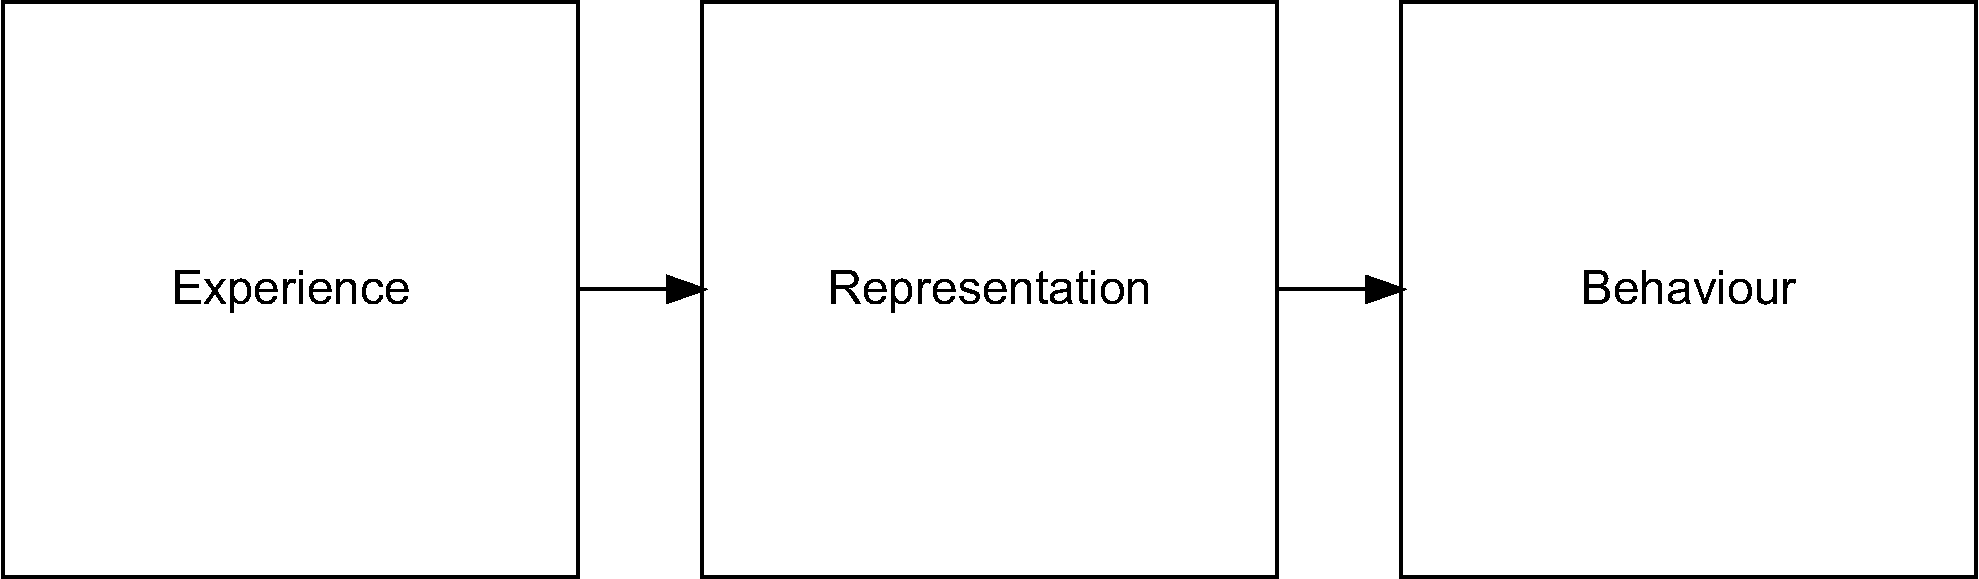
\includegraphics{Enrichment_files/figure-latex/Figure1-1.pdf}
\caption{\label{fig:Figure1}The process of translating experiences into behaviour via reprepresentation. Arrows represent processes that translate one domain into another. Thus learning translates experience into a representation and additional cognitive processes, such as associative recall, or similarity evaluations translate representations into behaviour.}
\end{figure}

\hypertarget{environment}{%
\subsection{Environment}\label{environment}}

The environment presents the set of possible relationships an individual could learn. It is represented here as network (matrix) cues, with the edges between cues indicating learnable associations. The environment presented here is a variation of fitness-based network model using rank-based sampling. This is inspired by the ubiquity of scaling laws in the cognitive sciences and the natural world (\textbf{Kello2010ga?}). This assumes a power-law relation in the frequency of cues: Each cue is assigned a rank, \(r\), from 1 to 1000. Then pairs of cues are chosen from the lexicon with probability \(p \propto r^{-a}\) and an edge is created between them. Here \(a\) is set to \(.1\) and 2000 edges are created. A scale-free network is not required to get the aging result shown below---for example, an Erdös-Renyi random graph produces the same qualitative pattern. In addition, the number of words available to learn could increase across the lifespan, as proposed by Brysbaert, Stevens, Mandera, and Keuleers (2016) and following \emph{Herdan-Heaps' law} (Petersen, Tenenbaum, Havlin, Stanley, \& Perc, 2012; Serrano, Flammini, \& Menczer, 2009). Again, the qualitative results are the same. Examples are provided in the Supplementary material.

\hypertarget{representation}{%
\subsection{Representation}\label{representation}}

Contemporary accounts characterize learning as minimizing prediction error, which is a fundamental assumption among models of reinforcement learning (Dayan \& Abbott, 2005; Hoppe, Hendriks, Ramscar, \& Rij, 2022; McClelland \& Rumelhart, 1981; Sutton \& Barto, 2018). The Rescorla-Wagner model (Rescorla \& Wagner, 1972) captures this phenomenology and is a model on which many subsequent models have been based (e.g., Sutton \& Barto, 1981; Trimmer, McNamara, Houston, \& Marshall, 2012). Moreover, it captures phenomenology like association learning, blocking, inhibition, and extinction.

The Rescorla-Wagner model formalizes learning as a process of minimizing prediction error between the values of an observed outcome, \(\lambda_j\) and a predictive cue, \(V_i\), where \(j\) and \(i\) represent specific outcomes and cues, respectively. The prediction error is the difference \((\lambda_j-V_i)\) and it is minimized following each learning event according to the following rule:

\[
\Delta V_{C \rightarrow U} = \alpha_C \beta_U (\lambda_{U} - V_{C \rightarrow U})
\]

\(\alpha\) corresponds to cue salience (some cues are easier to learn about than others) and \(\beta\) to the learning rate (some outcomes are learned about faster than others). Both \(\alpha\) and \(\beta\) values are confined to values between \(0\) and \(1\). After learning at time \(t\), the updated cue value is

\[
V_{C \rightarrow U, t+1} = V_{C \rightarrow U, t} + \Delta V_{C \rightarrow U, t}
\]

Here we allow the representation to be formed by learning from the environment over the lifetime. To do this, we allow learning to take place over four epochs, each with 500 learning events. Each learning event randomly samples a relationship from the environment represented as an edge in the environment network. Then one of the associates is randomly assigned as the cue and the other as the outcome, and the representation is updated according to the Rescorla-Wagner model with \(\alpha=1\) and \(\beta=.2\) and \(\lambda_i=1\).

\hypertarget{behaviour}{%
\subsection{Behaviour}\label{behaviour}}

The two stylized facts associated with cognitive aging are rising entropy and a reduction in pairwise similarity judgments. Each of these is recovered from the representation as follows.

\hypertarget{rising-entropy}{%
\subsubsection{Rising entropy}\label{rising-entropy}}

Rising entropy refers to the reduction in the predictability of free association targets as individuals age (Dubossarsky et al., 2017). We can measure this using \emph{Shannon's information entropy}. This measures the surprisingness of associate given the presence of a cue. Because the output of Rescorla-Wagner learning is a weighted edge, we can compute this for every cue in the network representation as follows:

\[
H = -\sum_{i=1}^{k}  p_i log(p_i)
\] Here, \(p_i\) is the proportion of the weight along edge \(i\) for all \(k\) edges. That is, \(p_i = \frac{w_i}{\sum_k w_k}\).

\hypertarget{similarity}{%
\subsubsection{Similarity}\label{similarity}}

To simulate similarity judgments, we will create a measure of co-activation between cues. To do this, we will allowing spreading activation to leave one node and measuring activation at the other node, \(A_{j \rightarrow k}\). This allows us to measure the extent to which one word co-activates the other. Doing this for both cues, we take similarity as the summed co-activation.

\[
S = A_{j \rightarrow k} + A_{j \rightarrow k}
\]

We will measure this similarity for all node pairs in the representation.

\hypertarget{results}{%
\section{Results}\label{results}}

\hypertarget{discussion}{%
\section{Discussion}\label{discussion}}

Because edges were formed in Dubossarsky et al. (2017) and Wulff et al. (2019) by requiring a minimun number of cue-target associations in the free association task, rising entropy corresponds to a less predictable pattern of cue-target associations and the lower likelihood of an edge between any cue-target pair. As a consequence, representational networks with higher entropy will produce behavioural networks that are more sparse.

Write some more stuff.

Do people who learn more showing earlier degradation? look at clutter paper.

Ramscar et al. (2014) suggested that ``older adults' changing performance reflects memory search demands, which escalate as experience grows'' (p.~5) because older adults largely show impaired paired-associated learning only for unrelated terms. In subsequent work,

\newpage

\hypertarget{references}{%
\section{References}\label{references}}

\hypertarget{refs}{}
\begin{CSLReferences}{1}{0}
\leavevmode\vadjust pre{\hypertarget{ref-amer2022cluttered}{}}%
Amer, T., Wynn, J. S., \& Hasher, L. (2022). Cluttered memory representations shape cognition in old age. \emph{Trends in Cognitive Sciences}, \emph{26}(3), 255--267.

\leavevmode\vadjust pre{\hypertarget{ref-boyle2021degree}{}}%
Boyle, P. A., Wang, T., Yu, L., Wilson, R. S., Dawe, R., Arfanakis, K., \ldots{} Bennett, D. A. (2021). To what degree is late life cognitive decline driven by age-related neuropathologies? \emph{Brain}, \emph{144}(7), 2166--2175.

\leavevmode\vadjust pre{\hypertarget{ref-brysbaert2016many}{}}%
Brysbaert, M., Stevens, M., Mandera, P., \& Keuleers, E. (2016). How many words do we know? Practical estimates of vocabulary size dependent on word definition, the degree of language input and the participant's age. \emph{Frontiers in Psychology}, \emph{7}(1116), 1--11.

\leavevmode\vadjust pre{\hypertarget{ref-buchler2007modeling}{}}%
Buchler, N. E., \& Reder, L. M. (2007). Modeling age-related memory deficits: A two-parameter solution. \emph{Psychology and Aging}, \emph{22}(1), 104.

\leavevmode\vadjust pre{\hypertarget{ref-cattell1987intelligence}{}}%
Cattell, R. B. (1987). \emph{Intelligence: Its structure, growth and action}. Elsevier.

\leavevmode\vadjust pre{\hypertarget{ref-cosgrove2021quantifying}{}}%
Cosgrove, A. L., Kenett, Y. N., Beaty, R. E., \& Diaz, M. T. (2021). Quantifying flexibility in thought: The resiliency of semantic networks differs across the lifespan. \emph{Cognition}, \emph{211}, 104631.

\leavevmode\vadjust pre{\hypertarget{ref-dayan2005theoretical}{}}%
Dayan, P., \& Abbott, L. F. (2005). \emph{Theoretical neuroscience: Computational and mathematical modeling of neural systems}. MIT Press.

\leavevmode\vadjust pre{\hypertarget{ref-deary2009age}{}}%
Deary, I. J., Corley, J., Gow, A. J., Harris, S. E., Houlihan, L. M., Marioni, R. E., \ldots{} Starr, J. M. (2009). Age-associated cognitive decline. \emph{British Medical Bulletin}, \emph{92}(1), 135--152.

\leavevmode\vadjust pre{\hypertarget{ref-desrosiers1986paired}{}}%
Desrosiers, G., \& Ivison, D. (1986). Paired associate learning: Normative data for differences between high and low associate word pairs. \emph{Journal of Clinical and Experimental Neuropsychology}, \emph{8}(6), 637--642.

\leavevmode\vadjust pre{\hypertarget{ref-dubossarsky2017quantifying}{}}%
Dubossarsky, H., De Deyne, S., \& Hills, T. (2017). Quantifying the structure of free association networks across the life span. \emph{Developmental Psychology}, \emph{53}(8), 1560--1570.

\leavevmode\vadjust pre{\hypertarget{ref-ge2002age}{}}%
Ge, Y., Grossman, R. I., Babb, J. S., Rabin, M. L., Mannon, L. J., \& Kolson, D. L. (2002). Age-related total gray matter and white matter changes in normal adult brain. Part i: Volumetric MR imaging analysis. \emph{American Journal of Neuroradiology}, \emph{23}(8), 1327--1333.

\leavevmode\vadjust pre{\hypertarget{ref-geerligs2015brain}{}}%
Geerligs, L., Renken, R. J., Saliasi, E., Maurits, N. M., \& Lorist, M. M. (2015). A brain-wide study of age-related changes in functional connectivity. \emph{Cerebral Cortex}, \emph{25}(7), 1987--1999.

\leavevmode\vadjust pre{\hypertarget{ref-giorgio2010age}{}}%
Giorgio, A., Santelli, L., Tomassini, V., Bosnell, R., Smith, S., De Stefano, N., \& Johansen-Berg, H. (2010). Age-related changes in grey and white matter structure throughout adulthood. \emph{Neuroimage}, \emph{51}(3), 943--951.

\leavevmode\vadjust pre{\hypertarget{ref-grady2006age}{}}%
Grady, C. L., Springer, M. V., Hongwanishkul, D., McIntosh, A. R., \& Winocur, G. (2006). Age-related changes in brain activity across the adult lifespan. \emph{Journal of Cognitive Neuroscience}, \emph{18}(2), 227--241.

\leavevmode\vadjust pre{\hypertarget{ref-hills2013mechanisms}{}}%
Hills, T., Mata, R., Wilke, A., \& Samanez-Larkin, G. R. (2013). Mechanisms of age-related decline in memory search across the adult life span. \emph{Developmental Psychology}, \emph{49}(12), 2396--2404.

\leavevmode\vadjust pre{\hypertarget{ref-hoppe2022exploration}{}}%
Hoppe, D. B., Hendriks, P., Ramscar, M., \& Rij, J. van. (2022). An exploration of error-driven learning in simple two-layer networks from a discriminative learning perspective. \emph{Behavior Research Methods}, \emph{54}(5), 2221--2251.

\leavevmode\vadjust pre{\hypertarget{ref-lemaitre2012normal}{}}%
Lemaitre, H., Goldman, A. L., Sambataro, F., Verchinski, B. A., Meyer-Lindenberg, A., Weinberger, D. R., \& Mattay, V. S. (2012). Normal age-related brain morphometric changes: Nonuniformity across cortical thickness, surface area and gray matter volume? \emph{Neurobiology of Aging}, \emph{33}(3), 617--e1.

\leavevmode\vadjust pre{\hypertarget{ref-mcclelland1981interactive}{}}%
McClelland, J. L., \& Rumelhart, D. E. (1981). An interactive activation model of context effects in letter perception: I. An account of basic findings. \emph{Psychological Review}, \emph{88}(5), 375--407.

\leavevmode\vadjust pre{\hypertarget{ref-park2009adaptive}{}}%
Park, D. C., \& Reuter-Lorenz, P. (2009). The adaptive brain: Aging and neurocognitive scaffolding. \emph{Annual Review of Psychology}, \emph{60}, 173--196.

\leavevmode\vadjust pre{\hypertarget{ref-petersen2012languages}{}}%
Petersen, A. M., Tenenbaum, J. N., Havlin, S., Stanley, H. E., \& Perc, M. (2012). Languages cool as they expand: Allometric scaling and the decreasing need for new words. \emph{Scientific Reports}, \emph{2}(943), 1--10.

\leavevmode\vadjust pre{\hypertarget{ref-ramscar2014myth}{}}%
Ramscar, M., Hendrix, P., Shaoul, C., Milin, P., \& Baayen, H. (2014). The myth of cognitive decline: Non-linear dynamics of lifelong learning. \emph{Topics in Cognitive Science}, \emph{6}(1), 5--42.

\leavevmode\vadjust pre{\hypertarget{ref-ramscar2017mismeasurement}{}}%
Ramscar, M., Sun, C. C., Hendrix, P., \& Baayen, H. (2017). The mismeasurement of mind: Life-span changes in paired-associate-learning scores reflect the {``cost''} of learning, not cognitive decline. \emph{Psychological Science}, \emph{28}(8), 1171--1179.

\leavevmode\vadjust pre{\hypertarget{ref-rescorla1972theory}{}}%
Rescorla, R. A., \& Wagner, A. R. (1972). {A theory of Pavlovian conditioning: Variations in the effectiveness of reinforcement and non-reinforcement}. In A. H. Prokasy (Ed.), \emph{Classical conditioning II: Current research and theory} (pp. 64--69). Appleton-Century-Crofts.

\leavevmode\vadjust pre{\hypertarget{ref-salthouse2013mechanisms}{}}%
Salthouse, T. A. (1992). \emph{Mechanisms of age-cognition relations in adulthood}. Lawrence Erlbaum Associates, Inc.

\leavevmode\vadjust pre{\hypertarget{ref-Salthouse:2004is}{}}%
Salthouse, T. A. (2004). {What and when of cognitive aging}. \emph{Current Directions in Psychological Science}, \emph{13}(4), 140--144.

\leavevmode\vadjust pre{\hypertarget{ref-Serrano:2009cv}{}}%
Serrano, M. Á., Flammini, A., \& Menczer, F. (2009). Modeling statistical properties of written text. \emph{PLoS ONE}, \emph{4}(4), e5372.

\leavevmode\vadjust pre{\hypertarget{ref-spreng2019shifting}{}}%
Spreng, R. N., \& Turner, G. R. (2019). The shifting architecture of cognition and brain function in older adulthood. \emph{Perspectives on Psychological Science}, \emph{14}(4), 523--542.

\leavevmode\vadjust pre{\hypertarget{ref-spreng2021exploration}{}}%
Spreng, R. N., \& Turner, G. R. (2021). From exploration to exploitation: A shifting mental mode in late life development. \emph{Trends in Cognitive Sciences}, \emph{25}(12), 1058--1071.

\leavevmode\vadjust pre{\hypertarget{ref-sutton1981toward}{}}%
Sutton, R. S., \& Barto, A. G. (1981). Toward a modern theory of adaptive networks: Expectation and prediction. \emph{Psychological Review}, \emph{88}(2), 135.

\leavevmode\vadjust pre{\hypertarget{ref-sutton2018reinforcement}{}}%
Sutton, R. S., \& Barto, A. G. (2018). \emph{Reinforcement learning: An introduction}. MIT Press.

\leavevmode\vadjust pre{\hypertarget{ref-trimmer2012does}{}}%
Trimmer, P. C., McNamara, J. M., Houston, A. I., \& Marshall, J. A. (2012). Does natural selection favour the rescorla--wagner rule? \emph{Journal of Theoretical Biology}, \emph{302}, 39--52.

\leavevmode\vadjust pre{\hypertarget{ref-wulff2022using}{}}%
Wulff, D. U., De Deyne, S., Aeschbach, S., \& Mata, R. (2022). Using network science to understand the aging lexicon: Linking individuals' experience, semantic networks, and cognitive performance. \emph{Topics in Cognitive Science}, \emph{14}(1), 93--110.

\leavevmode\vadjust pre{\hypertarget{ref-wulff2019new}{}}%
Wulff, D. U., De Deyne, S., Jones, M. N., \& Mata, R. (2019). New perspectives on the aging lexicon. \emph{Trends in Cognitive Sciences}, \emph{23}(8), 686--698.

\leavevmode\vadjust pre{\hypertarget{ref-zortea2014graph}{}}%
Zortea, M., Menegola, B., Villavicencio, A., \& Salles, J. F. de. (2014). Graph analysis of semantic word association among children, adults, and the elderly. \emph{Psicologia: Reflexao e Critica}, \emph{27}, 90--99.

\end{CSLReferences}


\end{document}
